\documentclass[a0,portrait]{a0poster}

\usepackage{multicol}
\columnsep=100pt
\columnseprule=3pt

\usepackage[svgnames]{xcolor}

\usepackage{times}
\usepackage{palatino}

\usepackage{graphicx}
\graphicspath{{figures/}}
\usepackage{booktabs}
\usepackage[font=small,labelfont=bf]{caption}
\usepackage{amsfonts, amsmath, amsthm, amssymb}
\usepackage{wrapfig}
\usepackage{lipsum,adjustbox}
\usepackage[absolute,overlay]{textpos}
\usepackage{multirow}
\usepackage{titlesec}
\usepackage{enumitem}
\usepackage{url}
\usepackage{tikz,pgfplots,pgfplotstable}
\usepackage{tikz-dependency}
\usetikzlibrary{arrows.meta}
\captionsetup{labelformat=empty}

\begin{document}

\begin{center}
	\veryHuge \color{NavyBlue} \textbf{Multitask Parsing Across Semantic Representations}
\end{center}
\vspace{-1cm}
\begin{minipage}[b]{.07\linewidth}

\includegraphics[width=\linewidth]{huji_logo.jpg}
\vspace{5mm}
\end{minipage}
\begin{minipage}[b]{.16\linewidth}

\includegraphics[width=\linewidth]{huji_banner.png}

\includegraphics[width=\linewidth]{cse_banner.jpg}
\vspace{.8mm}
\end{minipage}
\hspace{1cm}
\begin{minipage}[b]{0.57\linewidth}
\LARGE \textbf{Daniel Hershcovich}\textsuperscript{1,2} \&
	   \textbf{Omri Abend}\textsuperscript{2} \&
	   \textbf{Ari Rappoport}\textsuperscript{2} \\[0.5cm]
\Large $^1$The Edmond and Lily Safra Center for Brain Sciences \\
  $^2$School of Computer Science and Engineering
  \setlength{\columnseprule}{0pt}
  \setlength\multicolsep{-20pt}
  \begin{multicols}{2}
  The Hebrew University of Jerusalem
  \large \texttt{\{danielh,oabend,arir\}@cs.huji.ac.il}
  \end{multicols}
\end{minipage}
\hfill
\begin{minipage}[b]{.09\linewidth}

\includegraphics[width=\linewidth]{elsc_logo.png}\vspace{5mm}

\includegraphics[width=\linewidth]{icrici_banner.png}
\end{minipage}

\vspace{1cm}
\titlespacing*{\section}{0pt}{8mm}{5mm}

%----------------------------------------------------------------------------------------

\begin{adjustbox}{margin=3mm,frame,minipage=.6\linewidth,center}
\Large\color{Navy}
Multitask learning allows a transition-based semantic parser
to generalize from multiple tasks,
improving UCCA parsing in challenging settings.
\end{adjustbox}


\begin{multicols}{2}


\color{Black}

\section*{Introduction}

Semantic parsing is important for natural language understanding.
Representation schemes vary,
but data is mostly \textbf{small}, \textbf{in-domain}, and in \textbf{English}.
We consider four schemes:
\begin{description}[nosep,labelsep=1em]
\item[\color{violet} UCCA.] Intuitive, cross-lingual, and modular semantic representation.
    \textit{Primary edges} form a tree; directed acyclic graph (DAG) due to \textit{remote edges} (dashed).
    Edge labels encode predicate-argument structure, semantic heads and inter-scene relations
    \cite{abend2013universal}.
\item[\color{teal} AMR.] Abstract graph on concepts and constants, implicit alignment to text tokens.
    Rooted DAG with node and edge labels.
    Encodes named entities, argument structure, semantic roles, word sense and co-reference
    \cite{banarescu2013abstract}.
\item[\color{blue} SDP.] Set of related bilexical DAG schemes (DM, PAS, PSD and CCD). \\
    We use \textbf{\color{blue} DM} (DELPH-IN MRS).
    Encodes predicate-argument structure \cite{oepen2016towards}.
\item[\color{purple} UD.] Cross-lingual syntactic bilexical tree.
    Encodes syntactic relations between words \cite{nivre2016universal}. \\
    UD$^{++}$ (Enhanced++ UD) adds and augments edges, creating a bilexical DAG \cite{SCHUSTER16.779}.
\end{description}

\begin{minipage}{.6\columnwidth}
  \color{violet}
  \begin{center}
    \begin{tikzpicture}[level distance=3cm, sibling distance=45mm, -{Latex[length=5mm]},
        every circle node/.append style={fill=violet}]
      \tikzstyle{word} = [font=\rmfamily,color=black]
      \node (ROOT) [circle] {}
        child {node (After) [word] {After} edge from parent node[above] {L}}
        child {node (graduation) [circle] {}
        {
          child {node [word] {graduation} edge from parent node[left] {P}}
        } edge from parent node[right] {H} }
        child {node [word] {,} edge from parent node[below] {U}}
        child {node (moved) [circle] {}
        {
          child {node (John) [word] {John} edge from parent node[left] {A}}
          child {node [word] {moved} edge from parent node[left] {P}}
          child {node [circle] {}
          {
            child {node [word] {to} edge from parent node[left] {R}}
            child {node [word] {Paris} edge from parent node[right] {C}}
          } edge from parent node[above] {A} }
        } edge from parent node[right] {H} }
        ;
      \draw[dashed,->] (graduation) to node [above] {A} (John);
    \end{tikzpicture}
  \captionof{figure}{Universal Conceptual Cognitive Annotation (UCCA).}
  \end{center}
\end{minipage}
\hfill
\begin{minipage}{.2\columnwidth}
  \begin{center}
  \vspace{-1cm}
  \begin{adjustbox}{margin=2mm,frame,scale=.8}
  \begin{tabular}{cl}
	  P & process \\
	  S & state \\
	  A & participant \\
	  L & linker \\
	  H & linked scene \\
	  C & center \\
	  E & elaborator \\
	  D & adverbial \\
	  R & relator \\
	  N & connector \\
	  U & punctuation \\
	  F & function unit \\
	  G & ground
  \end{tabular}
  \end{adjustbox}
  \captionof{table}{UCCA edge labels.}
  \end{center}
\end{minipage}
\hrule
\begin{minipage}{.45\columnwidth}
  \begin{center}
  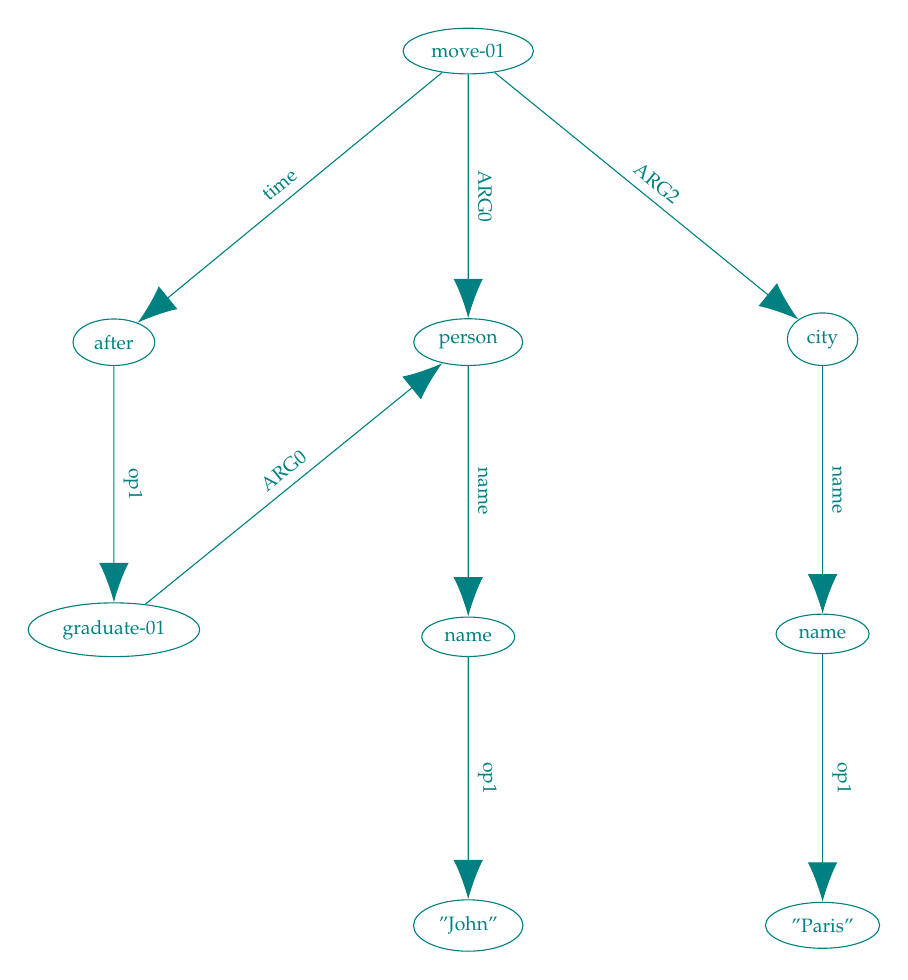
\begin{tikzpicture}[-{Latex[length=5mm]}, color=teal, level distance=4cm,
      every node/.append style={sloped,anchor=south,auto=false,font=\scriptsize},
      level 1/.style={sibling distance=45mm}]
    \node (ROOT) [draw=teal,ellipse] {move-01}
      child {node [draw=teal,ellipse] {after}
      {
            child {node (graduation) [draw=teal,ellipse] {graduate-01} edge from parent node {op1} }
      } edge from parent node {time} }
      child {node (John) [draw=teal,ellipse] {person}
      {
        child {node [draw=teal,ellipse] {name}
        {
            child {node [draw=teal,ellipse] {"John"} edge from parent node {op1} }
        } edge from parent node {name} }
      } edge from parent node {ARG0} }
      child {node [draw=teal,ellipse] {city}
      {
        child {node [draw=teal,ellipse] {name}
        {
            child {node [draw=teal,ellipse] {"Paris"} edge from parent node {op1} }
        } edge from parent node {name} }
      } edge from parent node {ARG2} }
      ;
      \draw (graduation) to node {ARG0} (John);
  \end{tikzpicture}
  \captionof{figure}{Abstract Meaning Representation (AMR).}
  \end{center}
\end{minipage}
\vrule
\begin{minipage}{.55\columnwidth}
    \begin{center}
    \begin{dependency}[edge style={-{Latex[length=4mm]}, color=blue},
        text only label, label style={above, color=blue}, font=\small]
    \begin{deptext}[column sep=.8em,ampersand replacement=\^]
    After \^ graduation \^ , \^ John \^ moved \^ to \^ Paris \\
    \end{deptext}
        \depedge[edge unit distance=1em]{1}{2}{ARG2}
        \depedge[edge unit distance=1em]{5}{4}{ARG1}
        \depedge[edge unit distance=1em, edge end x offset=-2mm]{1}{5}{ARG1}
        \deproot[edge unit distance=1.5em]{5}{top}
        \depedge[edge unit distance=2em, edge start x offset=-1mm, edge end x offset=3mm]{5}{7}{ARG2}
        \depedge[edge unit distance=1em, edge end x offset=5mm]{6}{5}{ARG1}
        \depedge[edge unit distance=1em]{6}{7}{ARG2}
    \end{dependency}
    \captionof{figure}{Semantic Dependencies (SDP): DM representation.}
    \hrule
    \vfill
    \begin{dependency}[edge style={-{Latex[length=4mm]}, color=purple},
        text only label, label style={above, color=purple}, font=\small]
    \begin{deptext}[column sep=.8em,ampersand replacement=\^]
    After \^ graduation \^ , \^ John \^ moved \^ to \^ Paris \\
    \end{deptext}
        \depedge[edge unit distance=1em]{2}{1}{case}
        \depedge[edge unit distance=1em]{4}{3}{punct}
        \depedge[edge unit distance=1em]{5}{4}{nsubj}
        \depedge[edge unit distance=1em, edge end x offset=-2mm]{2}{5}{obl}
        \depedge[edge unit distance=1em]{7}{6}{case}
        \deproot[edge unit distance=1em]{5}{root}
        \depedge[edge unit distance=1.5em]{5}{7}{obl}
    \end{dependency}
  \captionof{figure}{Universal Dependencies (UD).}
  \end{center}
\end{minipage}

While formally different, semantic representations
share much of their content \cite{abend2017state}.
We use multitask learning to exploit the task overlap
and effectively extend the training data
for a general transition-based DAG parser,
showing benefits for UCCA parsing.\footnote{Code:
\url{http://github.com/danielhers/tupa} \hfill
Corpora: \url{http://github.com/huji-nlp/ucca-corpora} \hfill
Implemented using DyNet: \url{http://github.com/clab/dynet}}

\hrule

\section*{General Transition-based DAG Parser}

We extend TUPA \cite{hershcovich2017a} to support
reentrancy, discontinuity and non-terminal nodes.

The parser applies a \textit{transition}
at each step to the parser state, comprising\\
$S$: working stack of nodes.
$B$: buffer of remaining nodes.
$G=(V,E,\ell)$: constructed graph.

\scalebox{.9}{
\begin{minipage}{.55\columnwidth}
	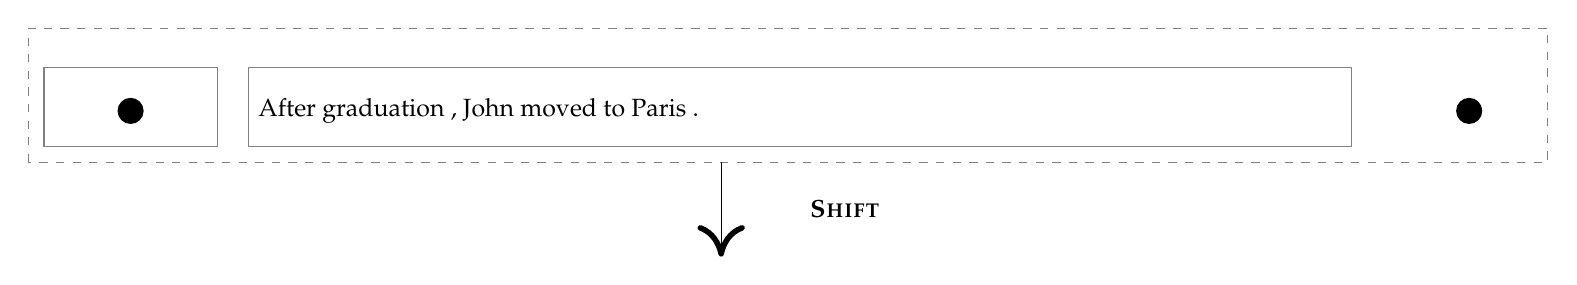
\begin{tikzpicture}[level distance=15mm, sibling distance=4cm, font=\small]
	\draw[color=gray,dashed] (.2,-.2) rectangle (19.5,1.5);
	\draw[color=gray] (.4,0) rectangle (2.6,1);
	\node[fill=black, circle] at (1.5,.45) {};
	\draw[color=gray] (3,0) rectangle (17,1);
	\node[anchor=west] at (3,.45) {After graduation , John moved to Paris .};
	\node[fill=black, circle] at (18.5,.45) {};
	\node[anchor=west] at (10,-.8) {\bf\small\textsc{Shift}};
	\draw[arrows={->[line width=2pt,length=4mm,width=6mm]}] (9,-.2) -- (9,-1.4);
	\end{tikzpicture}
	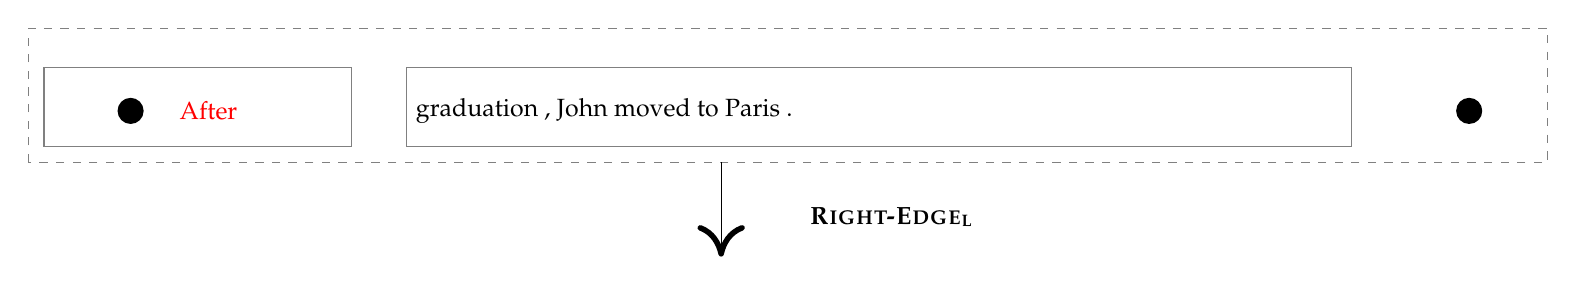
\begin{tikzpicture}[level distance=15mm, sibling distance=4cm, font=\small]
	\draw[color=gray,dashed] (.2,-.2) rectangle (19.5,1.5);
	\draw[color=gray] (.4,0) rectangle (4.3,1);
	\node[fill=black, circle] at (1.5,.45) {};
	\node[color=red,anchor=west] at (2,.45) {After};
	\draw[color=gray] (5,0) rectangle (17,1);
	\node[anchor=west] at (5,.45) {graduation , John moved to Paris .};
	\node[fill=black, circle] at (18.5,.45) {};
	\node[anchor=west] at (10,-.9) {\bf\small\textsc{Right-Edge\textsubscript L}};
	\draw[arrows={->[line width=2pt,length=4mm,width=6mm]}] (9,-.2) -- (9,-1.4);
	\end{tikzpicture}
	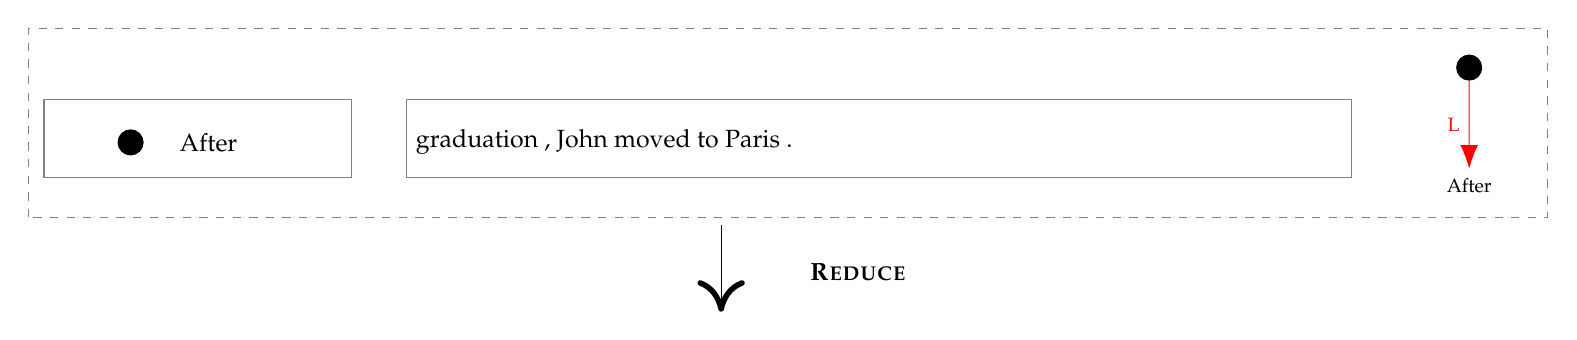
\begin{tikzpicture}[level distance=15mm, sibling distance=4cm, font=\small, -{Latex[length=3mm]}]
	\draw[color=gray,dashed] (.2,-.5) rectangle (19.5,1.9);
	\draw[color=gray] (.4,0) rectangle (4.3,1);
	\node[fill=black, circle] at (1.5,.45) {};
	\node[anchor=west] at (2,.45) {After};
	\draw[color=gray] (5,0) rectangle (17,1);
	\node[anchor=west] at (5,.45) {graduation , John moved to Paris .};
	\node[fill=black, circle] at (18.5,1.4) {}
	  child {node[font=\scriptsize] {After} edge from parent [red] node[font=\scriptsize,left] {L}};
	\node[anchor=west] at (10,-1.2) {\bf\small\textsc{Reduce}};
	\draw[arrows={->[line width=2pt,length=4mm,width=6mm]}] (9,-.6) -- (9,-1.7);
	\end{tikzpicture}
	\begin{tikzpicture}[level distance=15mm, sibling distance=4cm, font=\small, -{Latex[length=3mm]}]
	\draw[color=gray,dashed] (.2,-.5) rectangle (19.5,1.9);
	\draw[color=gray] (.4,0) rectangle (3,1);
	\node[fill=black, circle] at (1.5,.45) {};
	\draw[color=gray] (5,0) rectangle (17,1);
	\node[anchor=west] at (5,.45) {graduation , John moved to Paris .};
	\node[fill=black, circle] at (18.5,1.4) {}
	  child {node[font=\scriptsize] {After} edge from parent node[font=\scriptsize,left] {L}};
	\node[anchor=west] at (10,-1.2) {\bf\small\textsc{Shift}};
	\draw[arrows={->[line width=2pt,length=4mm,width=6mm]}] (9,-.6) -- (9,-1.7);
	\end{tikzpicture}
	\begin{tikzpicture}[level distance=15mm, sibling distance=4cm, font=\small, -{Latex[length=3mm]}]
	\draw[color=gray,dashed] (.2,-.5) rectangle (19.5,1.9);
	\draw[color=gray] (.4,0) rectangle (6,1);
	\node[fill=black, circle] at (1.5,.45) {};
	\node[color=red,anchor=west] at (2,.45) {graduation};
	\draw[color=gray] (8.5,0) rectangle (17,1);
	\node[anchor=west] at (8.8,.45) {, John moved to Paris .};
	\node[fill=black, circle] at (18.5,1.4) {}
	  child {node[font=\scriptsize] {After} edge from parent node[font=\scriptsize,left] {L}};
	\node[anchor=west] at (10,-1.2) {\bf\small\textsc{Node\textsubscript P}};
	\draw[arrows={->[line width=2pt,length=4mm,width=6mm]}] (9,-.6) -- (9,-1.7);
	\end{tikzpicture}
	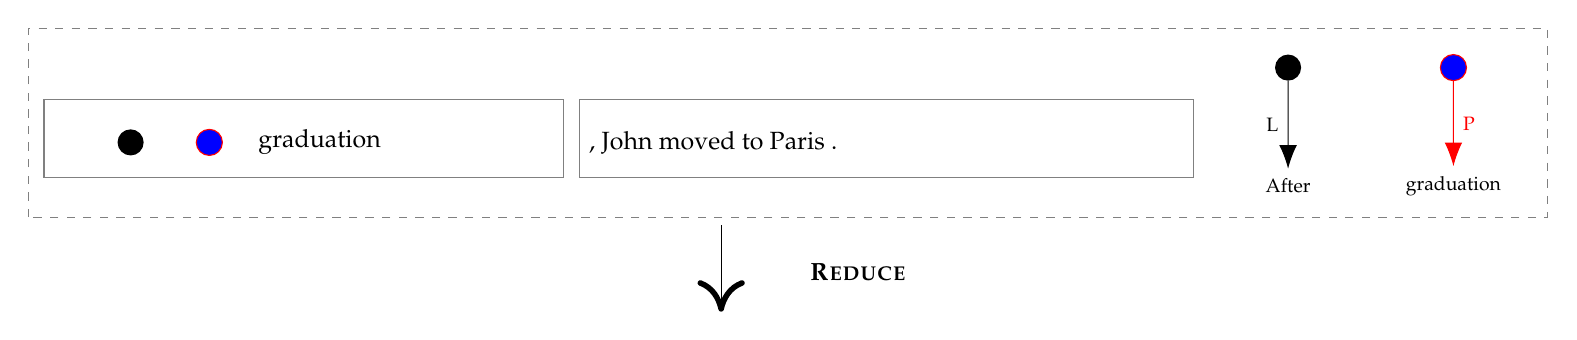
\begin{tikzpicture}[level distance=15mm, sibling distance=4cm, font=\small, -{Latex[length=3mm]}]
	\draw[color=gray,dashed] (.2,-.5) rectangle (19.5,1.9);
	\draw[color=gray] (.4,0) rectangle (7,1);
	\node[fill=black, circle] at (1.5,.45) {};
	\node[fill=blue, draw=red, circle] at (2.5,.45) {};
	\node[anchor=west] at (3,.45) {graduation};
	\draw[color=gray] (7.2,0) rectangle (15,1);
	\node[anchor=west] at (7.2,.45) {, John moved to Paris .};
	\node[fill=black, circle] at (16.2,1.4) {}
	  child {node[font=\scriptsize] {After} edge from parent node[font=\scriptsize,left] {L}};
	\node[fill=blue, draw=red, circle] at (18.3,1.4) {}
	  child {node[font=\scriptsize] {graduation} edge from parent [red] node[font=\scriptsize,right] {P}};
	\node[anchor=west] at (10,-1.2) {\bf\small\textsc{Reduce}};
	\draw[arrows={->[line width=2pt,length=4mm,width=6mm]}] (9,-.6) -- (9,-1.7);
	\end{tikzpicture}
\end{minipage}
\hspace{1cm}
\begin{minipage}{.4\columnwidth}
	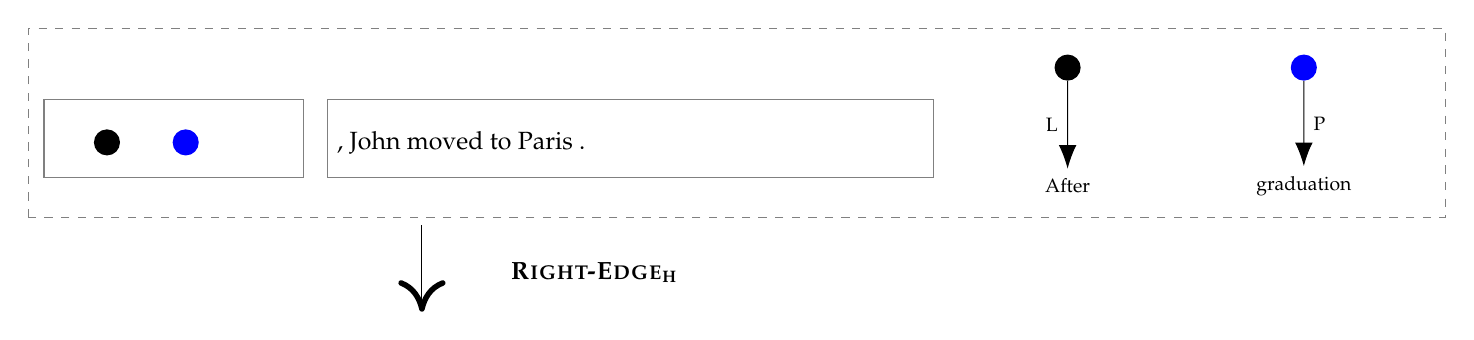
\begin{tikzpicture}[level distance=15mm, sibling distance=4cm, font=\small, -{Latex[length=3mm]}]
	\draw[color=gray,dashed] (0,-.5) rectangle (18,1.9);
	\draw[color=gray] (0.2,0) rectangle (3.5,1);
	\node[fill=black, circle] at (1,.45) {};
	\node[fill=blue, circle] at (2,.45) {};
	\draw[color=gray] (3.8,0) rectangle (11.5,1);
	\node[anchor=west] at (3.8,.45) {, John moved to Paris .};
	\node[fill=black, circle] at (13.2,1.4) {}
	  child {node[font=\scriptsize] {After} edge from parent node[font=\scriptsize,left] {L}};
	\node[fill=blue, circle] at (16.2,1.4) {}
	  child {node[font=\scriptsize] {graduation} edge from parent node[font=\scriptsize,right] {P}};
	\node[anchor=west] at (6,-1.2) {\bf\small\textsc{Right-Edge\textsubscript H}};
	\draw[arrows={->[line width=2pt,length=4mm,width=6mm]}] (5,-.6) -- (5,-1.7);
	\end{tikzpicture}
	\begin{tikzpicture}[level distance=15mm, sibling distance=4cm, font=\small, -{Latex[length=3mm]}]
	\draw[color=gray,dashed] (0,-1.9) rectangle (18,1.9);
	\draw[color=gray] (0.2,0) rectangle (3.5,1);
	\node[fill=black, circle] at (1,.45) {};
	\node[fill=blue, circle] at (2,.45) {};
	\draw[color=gray] (3.8,0) rectangle (11.5,1);
	\node[anchor=west] at (3.8,.45) {, John moved to Paris .};
	\node[fill=black, circle] at (14.7,1.4) {}
	  child {node[font=\scriptsize] {After} edge from parent node[font=\scriptsize,left] {L}}
	  child {node [fill=blue, circle] {}
	  {
	    child {node[font=\scriptsize] {graduation} edge from parent [black] node[font=\scriptsize,right] {P}}
	  } edge from parent [red] node[font=\scriptsize,right] {H} };
	\node[anchor=west] at (6,-2.5) {\bf\small\textsc{Shift}};
	\draw[arrows={->[line width=2pt,length=4mm,width=6mm]}] (5,-1.9) -- (5,-3);
	\end{tikzpicture}
	\begin{tikzpicture}[level distance=15mm, sibling distance=4cm, font=\small, -{Latex[length=3mm]}]
	\draw[color=gray,dashed] (0,-1.9) rectangle (18,1.9);
	\draw[color=gray] (0.2,0) rectangle (3.6,1);
	\node[fill=black, circle] at (1,.45) {};
	\node[fill=blue, circle] at (2,.45) {};
	\node[color=red, anchor=west] at (3,.25) {,};
	\draw[color=gray] (3.9,0) rectangle (11.5,1);
	\node[anchor=west] at (3.9,.45) {John moved to Paris .};
	\node[fill=black, circle] at (14.7,1.4) {}
	  child {node[font=\scriptsize] {After} edge from parent node[font=\scriptsize,left] {L}}
	  child {node [fill=blue, circle] {}
	  {
	    child {node[font=\scriptsize] {graduation} edge from parent node[font=\scriptsize,right] {P}}
	  } edge from parent node[font=\scriptsize,right] {H} };
	\node[anchor=west] at (6,-2.5) {\Large \ldots};
	\draw[arrows={->[line width=2pt,length=4mm,width=6mm]}] (5,-1.9) -- (5,-3);
	\end{tikzpicture}
	\begin{tikzpicture}[level distance=15mm, sibling distance=3cm, font=\small, -{Latex[length=3mm]}]
	\draw[color=gray,dashed] (0,-4) rectangle (18,2.2);
	\draw[color=gray] (.2,0) rectangle (1,1);
	\draw[color=gray] (1.3,0) rectangle (2,1);
    \node (ROOT) [fill=black,circle] at (8,1.5) {}
      child {node[font=\scriptsize] (After) {After} edge from parent node[font=\scriptsize,left] {L}}
      child {node (graduation) [fill=blue,circle] {}
      {
        child {node[font=\scriptsize] {graduation} edge from parent node[font=\scriptsize,left] {P}}
      } edge from parent node[font=\scriptsize,left] {H} }
      child {node[font=\scriptsize] {,} edge from parent node[font=\scriptsize,right] {U}}
      child {node (moved) [fill=purple,circle] {}
      {
        child {node[font=\scriptsize] (John) {John} edge from parent node[font=\scriptsize,left] {A}}
        child {node[font=\scriptsize] {moved} edge from parent node[font=\scriptsize,left] {P}}
        child {node [fill=orange,circle] {}
        {
          child {node[font=\scriptsize] {to} edge from parent node[font=\scriptsize,left] {R}}
          child {node[font=\scriptsize] {Paris} edge from parent node[font=\scriptsize,right] {C}}
        } edge from parent node[font=\scriptsize,right] {A} }
      } edge from parent node[font=\scriptsize,right] {H} }
      ;
    \draw[dashed] (graduation) to node [font=\scriptsize,auto] {A} (John);
	\end{tikzpicture}
\end{minipage}
}
\captionof{figure}{Example for intermediate states during transition-based UCCA parsing.}
\vspace{5mm}

A classifier selects the next transition based on the current state's features,
trained by an oracle based on gold-standard annotations.
Architecture: bidirectional LSTM RNN to encode features + feedforward NN for classification.


\hrule

\section*{Unified DAG Format}

We convert all four representations into a format similar to UCCA,
supported by the TUPA transition set.

\begin{minipage}{.4\columnwidth}
  \begin{center}
  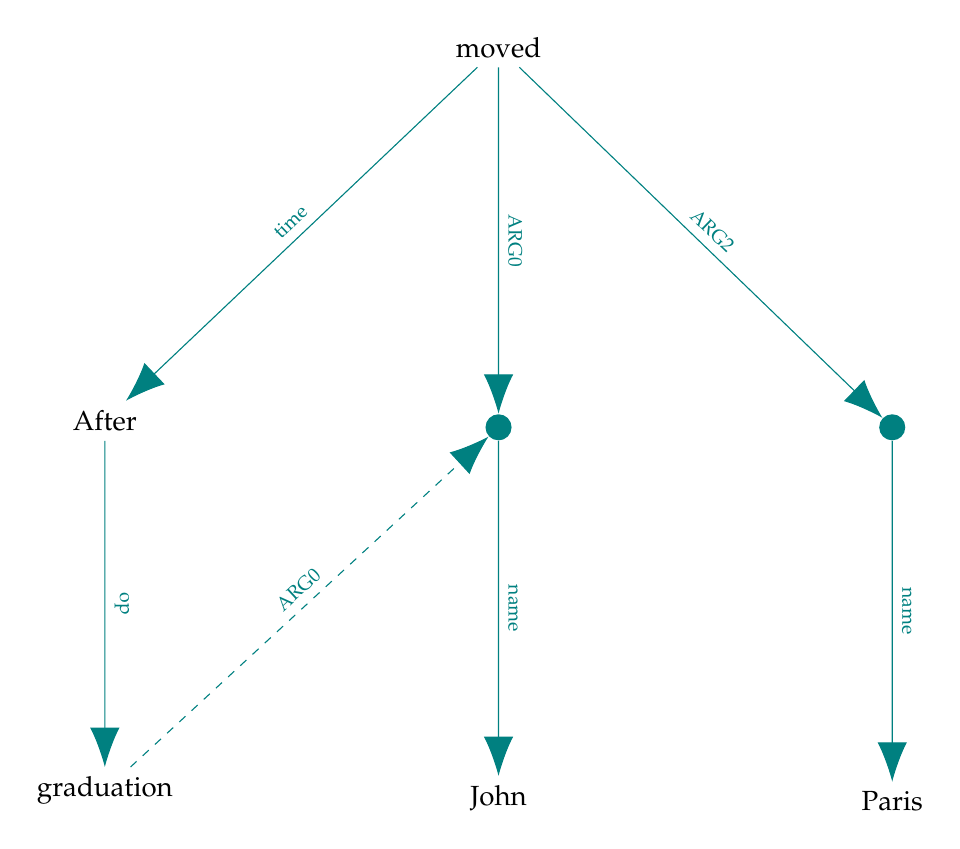
\begin{tikzpicture}[level distance=5cm, -{Latex[length=5mm]}, color=teal,
      every node/.append style={sloped,anchor=south,auto=false,font=\scriptsize},
      level 1/.style={sibling distance=5cm},
      level 2/.style={sibling distance=3cm},
      level 3/.style={sibling distance=3cm}]
    \tikzstyle{word} = [font=\rmfamily,color=black]
    \node (ROOT) [word] {moved}
      child {node [word] {After}
      {
            child {node (graduation) [word] {graduation} edge from parent node {op} }
      } edge from parent node {time} }
      child {node (John) [fill=teal,circle] {}
      {
        child {node [word] {John} edge from parent node {name} }
      } edge from parent node {ARG0} }
      child {node [fill=teal,circle] {}
      {
        child {node [word] {Paris} edge from parent node {name} }
      } edge from parent node {ARG2} }
      ;
      \draw[dashed] (graduation) to node {ARG0} (John);
  \end{tikzpicture}
  \captionof{figure}{Converted AMR.}
  \end{center}
\end{minipage}
\vrule
\begin{minipage}{.6\columnwidth}
  \begin{center}
  \scalebox{.9}{
  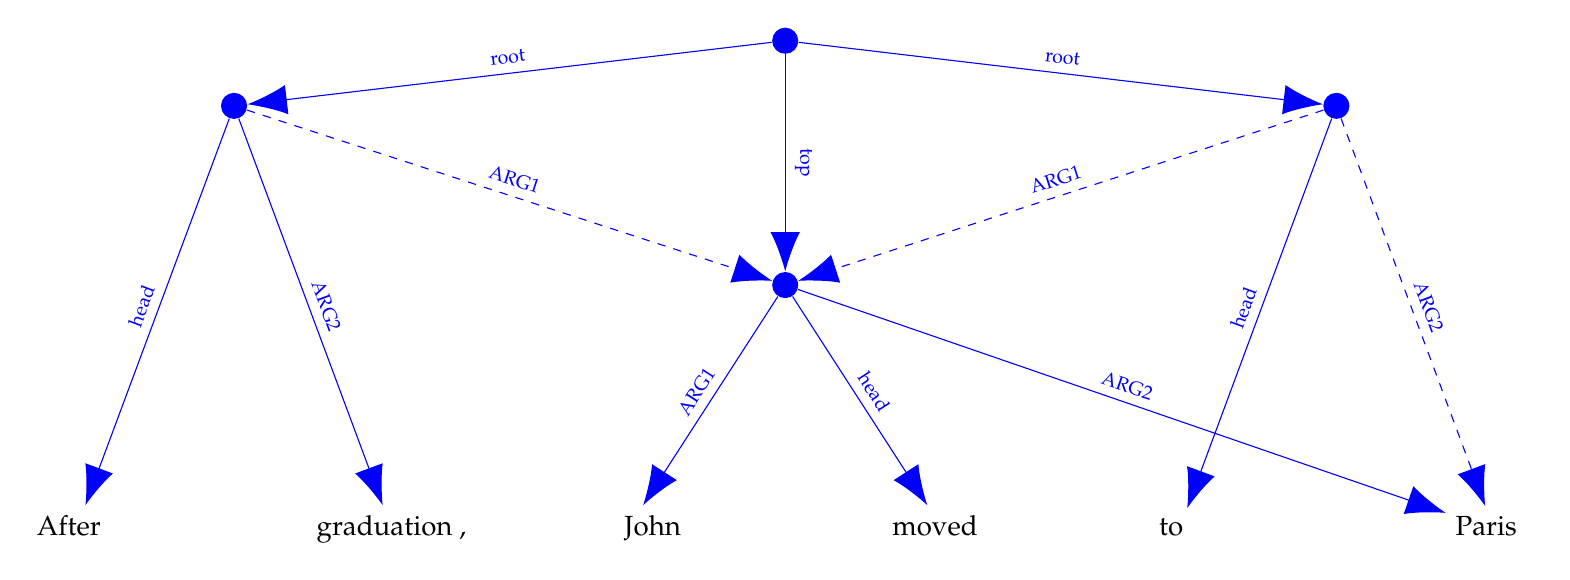
\begin{tikzpicture}[-{Latex[length=5mm]}, color=blue,
      every node/.append style={sloped,anchor=south,auto=false,font=\scriptsize},
      level 1/.style={sibling distance=7cm,level distance=1cm},
      level 2/.style={sibling distance=4cm,level distance=24mm},
      level 3/.style={level distance=34mm}]
    \tikzstyle{word} = [font=\rmfamily,color=black]
    \node (ROOT) [fill=blue,circle] {}
      child {node (after) [fill=blue,circle] {}
      {
        child {node [draw=none] {}
        {
          child {node [word] (after_word) {After{\color{white}g}} edge from parent [draw=none]}
        } edge from parent [draw=none] }
        child {node [draw=none] {}
        {
          child {node [word] (graduation) {graduation ,} edge from parent [draw=none]}
        } edge from parent [draw=none] }
      } edge from parent node {root}}
      child {node [draw=none] {}
      {
        child {node (moved) [fill=blue,circle] {}
        {
          child {node [word] {\quad{\color{white}g} John} edge from parent node {ARG1}}
          child {node [word] {moved{\color{white}g}} edge from parent node {head}}
        } edge from parent [draw=none] }
      } edge from parent [draw=none] }
      child {node (to) [fill=blue,circle] {}
      {
        child {node [draw=none] {}
        {
            child {node [word] (to_word) {to{\color{white}g}} edge from parent [draw=none]}
          } edge from parent [draw=none] }
          child {node [draw=none] {}
        {
          child {node [word] (Paris) {Paris{\color{white}g}} edge from parent [draw=none]}
        } edge from parent [draw=none] }
      } edge from parent node {root}}
      ;
      \draw (ROOT) to node {top} (moved);
      \draw (after) to node {head} (after_word);
      \draw (after) to node {ARG2} (graduation);
      \draw[dashed] (after) to node {ARG1} (moved);
      \draw[dashed] (to) to node {ARG1} (moved);
      \draw (to) to node {head} (to_word);
      \draw (moved) to node {ARG2} (Paris);
      \draw[dashed] (to) to node {ARG2} (Paris);
  \end{tikzpicture}}
  \captionof{figure}{Converted DM.}
  \hrule
  \scalebox{.9}{
  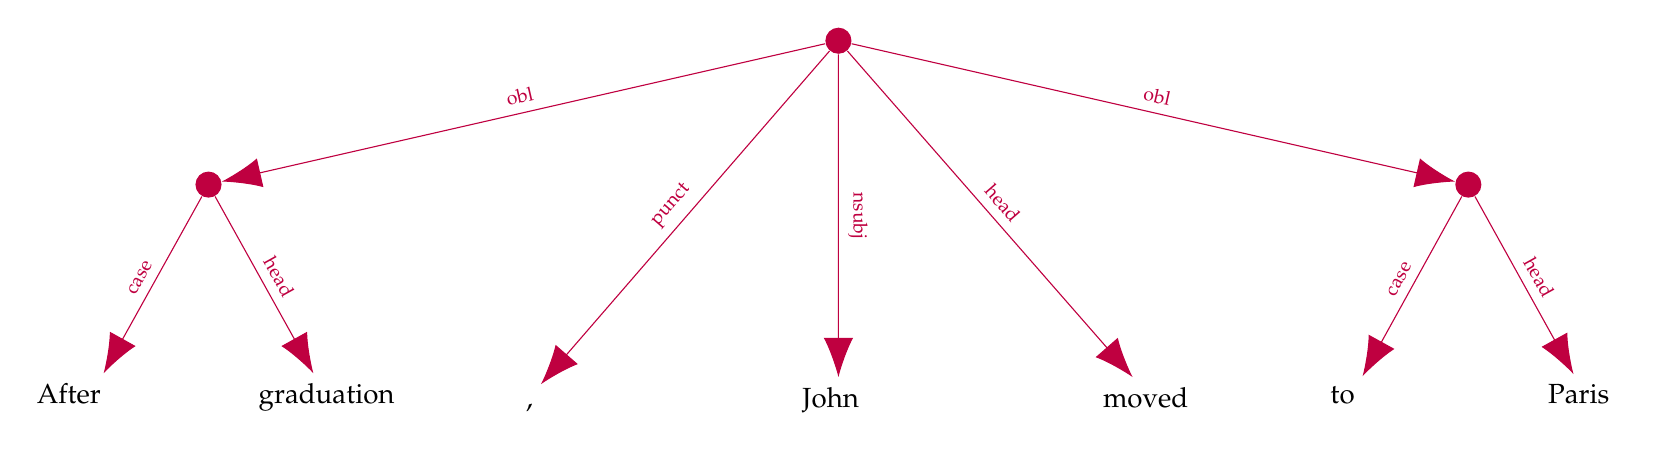
\begin{tikzpicture}[-{Latex[length=5mm]}, color=purple,
      every node/.append style={sloped,anchor=south,auto=false,font=\scriptsize},
      level 1/.style={sibling distance=4cm,level distance=2cm},
      level 2/.style={sibling distance=3cm,level distance=3cm}]
    \tikzstyle{word} = [font=\rmfamily,color=black]
    \node (ROOT) [fill=purple,circle] {}
      child {node (after) [fill=purple,circle] {}
      {
        child {node [word] {After{\color{white}g}\quad\quad} edge from parent node {case}}
        child {node [word] {\quad graduation\quad\quad} edge from parent node {head}}
      } edge from parent node {obl}}
      child {node {}
      {
        child {node [word] (comma) {\quad,{\color{white}g}} edge from parent [draw=none]}
      } edge from parent [draw=none]}
      child {node {}
      {
        child {node [word] (John) {John{\color{white}g}} edge from parent [draw=none]}
      } edge from parent [draw=none]}
      child {node {}
      {
        child {node [word] (moved) {moved{\color{white}g}} edge from parent [draw=none]}
      } edge from parent [draw=none]}
      child {node (to) [fill=purple,circle] {}
      {
          child {node [word] {to{\color{white}g}} edge from parent node {case}}
          child {node [word] {Paris{\color{white}g}} edge from parent node {head}}
      } edge from parent node {obl}}
      ;
      \draw (ROOT) to node {punct} (comma);
      \draw (ROOT) to node {nsubj} (John);
      \draw (ROOT) to node {head} (moved);
  \end{tikzpicture}}
  \captionof{figure}{Converted UD.}
  \end{center}
\end{minipage}

\hrule

\section*{Multitask Architecture}

We use a task-specific BiLSTM for each task, add
a BiLSTM that is shared across all tasks,
concatenate their outputs and choose a transition using
a task-specific MLP.
Feature embeddings are shared across tasks.
\begin{center}
   \begin{tikzpicture}[-{Latex[length=2mm]},level distance=15mm, sibling distance=3cm]
   \node[anchor=west] at (0,2.5) {Parser state};
   \draw[color=gray,dashed] (0,-.8) rectangle (22.5,3.75);
   \draw[color=gray] (.3,0) rectangle (4.5,1.5);
   \node[fill=black, circle] at (1.2,.875) {};
   \node[fill=blue, circle] at (2.7,.875) {};
   \node[anchor=west] at (3.75,.575) {,};
   \draw[color=gray] (5.95,0) rectangle (14.9,1.5);
   \node[anchor=west] at (5.95,.875) {John moved to Paris .};
   \node[fill=black, circle] at (19,2.75) {}
     child {node[font=\scriptsize] {After} edge from parent node[font=\scriptsize,left] {L}}
     child {node [fill=blue, circle] {}
     {
       child {node[font=\scriptsize] {graduation} edge from parent node[font=\scriptsize,right] {P}}
     } edge from parent node[font=\scriptsize,right] {H} };
   \end{tikzpicture}
   
   \begin{tikzpicture}[-{Latex[length=2mm]}]
   \node[anchor=west] at (0,17) {Classifier};
   \tikzstyle{main}=[rounded rectangle, minimum size=15mm, draw=black!80, node distance=12mm]
   \node[main] (specific) at (4,9) {Task-specific BiLSTM};
   \node[main,color=blue] (shared) at (18,9) {Shared BiLSTM};
   \node[color=blue] (embeddings) at (10.5,3) {Shared embeddings};
   \foreach \i/\word in {0/{After},6/{graduation},15/{to},21/{Paris}} {
       \node (x\i) at (\i,1) {\word};
       \node[main,color=blue] (e\i) at (\i,5) {};
       \path[color=blue] (x\i) edge (e\i);
       \path (e\i) edge (specific);
       \path[color=blue] (e\i) edge (shared);
   }
    \node (x4) at (10.5,2) {\ldots};
    \node[main] (mlp) at (10.5,12) {Task-specific MLP};
    \path (specific) edge (mlp);
    \path[color=blue] (shared) edge (mlp);
    \coordinate (state) at (19,18);
    \path (state) edge [bend left] (mlp);
    \node (transition) at (10.5,16.4) {transition};
    \path (mlp) edge node[right] {softmax} (transition);
   \end{tikzpicture}
   \captionof{figure}{Multitask model.}
\end{center}

We focus on UCCA due to its small training set, using AMR, SDP and UD as auxiliaries,
for which we perform unlabeled parsing,
resulting in a set of $\leq$10 transitions (45 for labeled UCCA parsing).
This limited capacity forces the network to use the shared parameters for all tasks,
increasing generalization \cite{E17-1005}.

\section*{Data}

\textbf{\color{violet} UCCA}: v1.2 of English Wikipedia corpus (Wiki);
\textit{Twenty Thousand Leagues Under the Sea} corpora (20K),
annotated in English (v1.0, small, only test) French (v1.0, small), and German (v0.9, pre-release, noisy).
\textbf{\color{teal} AMR}: LDC2017T10.
\textbf{\color{blue} SDP}: DM part from SDP 2016.
\textbf{\color{purple} UD}: all English, French and German treebanks, v2.1 (UD$^{++}$ for English).

While UCCA is annotated over Wikipedia and over a literary corpus,
the domains for AMR, DM and UD are blogs, news, emails, reviews, and Q\&A.

Number of sentences per dataset:

\begin{minipage}{.43\columnwidth}
\pgfplotstableread[row sep=\\,col sep=&]{
	corpus & train & dev & test \\
	UD & 17062 & 0 & 0 \\
	SDP & 33964 & 0 & 0 \\
	AMR & 36521 & 0 & 0 \\
	UCCA (Wiki) & 4268 & 454 & 503 \\
	UCCA (20K) & 0 & 0 & 506 \\
    }\english
\begin{center}
    \begin{tikzpicture}
    \begin{axis}[
    xbar stacked,
    xmin=0,
    xtick=\empty,
    ytick=data,
    yticklabels from table={\english}{corpus}
    ]
    \addplot [fill=green!80] table [x=train, meta=corpus,y expr=\coordindex] {\english};
    \addplot [fill=blue!60] table [x=dev, meta=corpus,y expr=\coordindex] {\english};
    \addplot [fill=red!60, point meta=x, nodes near coords, nodes near coords align={anchor=west},
    every node near coord/.append style={
        black,
        fill=white,
        fill opacity=0.75,
        text opacity=1,
        outer sep=\pgflinewidth
    }
    ] table [x=test, meta=corpus,y expr=\coordindex] {\english};
    \end{axis}
    \end{tikzpicture}
    \captionof{figure}{English.}
\end{center}
\end{minipage}
\begin{minipage}{.26\columnwidth}
\pgfplotstableread[row sep=\\,col sep=&]{
	corpus & train & dev & test \\
	UD & 32347 & 0 & 0 \\
	UCCA 20K & 413 & 67 & 67 \\
    }\french
\begin{center}
    \begin{tikzpicture}
    \begin{axis}[
    xbar stacked,
    xmin=0,
    xtick=\empty,
    ytick=\empty,
    yticklabels=\empty
    ]
    \addplot [fill=green!80] table [x=train, meta=corpus,y expr=\coordindex] {\french};
    \addplot [fill=blue!60] table [x=dev, meta=corpus,y expr=\coordindex] {\french};
    \addplot [fill=red!60, point meta=x, nodes near coords, nodes near coords align={anchor=west},
    every node near coord/.append style={
        black,
        fill=white,
        fill opacity=0.75,
        text opacity=1,
        outer sep=\pgflinewidth
    }
    ] table [x=test, meta=corpus,y expr=\coordindex] {\french};
    \end{axis}
    \end{tikzpicture}
    \captionof{figure}{French.}
\end{center}
\end{minipage}
\begin{minipage}{.3\columnwidth}
\pgfplotstableread[row sep=\\,col sep=&]{
	corpus & train & dev & test \\
	UD & 13814 & 0 & 0 \\
	UCCA 20K & 3429 & 561 & 2164 \\
    }\german
\begin{center}
    \begin{tikzpicture}
    \begin{axis}[
    xbar stacked,
    xmin=0,
    xtick=\empty,
    ytick=\empty,
    legend style={at={(axis cs:8000,.8)},anchor=north west},
    yticklabels=\empty
    ]
    \addplot [fill=green!80] table [x=train, meta=corpus,y expr=\coordindex] {\german};
    \addplot [fill=blue!60] table [x=dev, meta=corpus,y expr=\coordindex] {\german};
    \addplot [fill=red!60, point meta=x, nodes near coords, nodes near coords align={anchor=west},
    every node near coord/.append style={
        black,
        fill=white,
        fill opacity=0.75,
        text opacity=1,
        outer sep=\pgflinewidth
    }
    ] table [x=test, meta=corpus,y expr=\coordindex] {\german};
    \legend{train,dev,test}
    \end{axis}
    \end{tikzpicture}
    \captionof{figure}{German.}
\end{center}
\end{minipage}


\hrule


\section*{Results}

Labeled precision, recall and $F_1$ (in~\%) for primary and remote edges
on the 20K test sets
($\star$~indicates significantly better than \textit{Single},
and $\dagger$ significantly worse):
\begin{center}
\setlength\tabcolsep{1cm}
\begin{tabular}{l|lll|lll}
& \multicolumn{3}{c|}{\bf Primary} & \multicolumn{3}{c}{\bf Remote} \\
& \textbf{LP} & \textbf{LR} & \textbf{LF}
& \textbf{LP} & \textbf{LR} & \textbf{LF} \\
\hline
\bf English (out-of-domain) & \\
TUPA \cite{hershcovich2017a}
& 68.7 & 68.5 & 68.6 & 38.6 & 18.8 & 25.3 \\
Our single (UCCA only)
& 68.9 & 68.9 & 68.9 & 40.7 & 19.6 & 26.5 \\
\cline{1-1}
+ AMR
& 69.4 & 69.6 & 69.5 & 44.3 & 21.4 & 28.8 \\
+ DM
& 70.1$\star$ & 69.5 & 69.8$\star$ & 40 & 18.6 & 25.4 \\
+ UD$^{++}$
& 69.8$\star$ & 69.4 & 69.6 & 39.8 & 14.7$\dagger$ & 21.4$\dagger$ \\
+ AMR + DM
& 69.8$\star$ & 69.5 & 69.7$\star$ & 48.8$\star$ & 19.6 & 28 \\
+ AMR + UD$^{++}$
& 69.7$\star$ & 70$\star$ & 69.8$\star$ & 39 & 21.4 & 27.6 \\
+ DM + UD$^{++}$
& 70$\star$ & 68.9 & 69.4 & 47.4$\star$ & 22 & 30$\star$ \\
+ AMR + DM + UD$^{++}$
& 71$\star$ & 72.2$\star$ & \textbf{71.6}$\star$ & 43.9 & 24.8$\star$ & \textbf{31.6}$\star$ \\
\hline
\bf French (in-domain) & \\
Our single (UCCA only) & 64.1 & 60.6 & 62.3 & 20 & \enskip 5.7 & \enskip 8.8 \\
+ UD & 68.7$\star$ & 68.6$\star$ & \textbf{68.6}$\star$ & 15.8 & \enskip 5.7 & \enskip 8.3 \\
\hline
\bf German (in-domain) & \\
Our single (UCCA only) & 73.3 & 71.7 & 72.5 & 57.1 & 17.7 & 27.1 \\
+ UD & 73.7$\star$ & 72.6$\star$ & \textbf{73.2}$\star$ & 61.8 & 24.9$\star$ & \textbf{35.5}$\star$
\end{tabular}
\captionof{table}{Experimental results.}
\end{center}

\hrule


\section*{Conclusion}

We demonstrate that multitask learning improves UCCA parsing in out-of-domain settings
or when training data is scarce or noisy,
using AMR, DM and UD parsing as auxiliaries,
by proposing a unified DAG representation,
constructing protocols for converting these schemes into the unified format,
and generalizing a transition-based DAG parser.

A natural question is whether our method can benefit AMR, SDP or UD.
Future work will investigate whether a single
algorithm and architecture can be competitive on all of these.

\color{DarkSlateGray}
\tiny
\bibliographystyle{plain}
\bibliography{references}

\end{multicols}
\end{document}
